% Preamble
% ---
\documentclass{article}

% Packages
% ---
\usepackage{amsmath} % Advanced math typesetting
\usepackage[utf8]{inputenc} % Unicode support (Umlauts etc.)
\usepackage[english, ngerman]{babel} % Change hyphenation rules
\usepackage{hyperref} % Add a link to your document
\usepackage{graphicx} % Add pictures to your document
\usepackage{listings} % Source code formatting and highlighting
\usepackage{csquotes}
\usepackage{makecell}
\usepackage{multirow}
\usepackage{diagbox}
\usepackage{booktabs, tabularx}
\usepackage{parskip}
\usepackage[backend=bibtex,style=verbose-trad2]{biblatex} % Use biblatex package
\bibliography{quick} % The name of the .bib file (name without .bib)
\usepackage{abstract}
%\usepackage[toc,page]{appendix}
\setlength{\absleftindent}{0mm}
\setlength{\absrightindent}{0mm}
\setlength{\parindent}{0mm}


% Main document
% ---

\begin{document}
\selectlanguage{english}
% Set up the maketitle command
\author{Georges Leschener M. Essomba}
\title{PhD end of Year 1 Probation report}
\date{18th September 2019} % You can remove \today{} and type a date manually

\maketitle{} % Generates title

\pagebreak % Start new page.
\tableofcontents % Generates table of contents from sections
\pagebreak % Start new page

%\renewcommand*\abstractname{\flushleft\textbf{Abstract}\hfill}



\section{Project overview}


Microservices are gaining more and more popularity as an architectural style for building modern applications. Unlike monolithic applications, microservices are loosely coupled components, that can be deployed and maintained independently and developed using different technologies. They do introduce a number of benefits including accelerating innovation given the speed at which applications can be built and new services taken to market. Agility in terms of how easily microservices can be modified, say for instance to adapt to a change in the market. Scale as microservices as cloud appears to be the preferred platform for deploying microservices, and one of the values that cloud computing does provide is elasticity and scale, and last but not least security. With microservices it is possible to provide fine-grain security access control by giving access to users to only part of the application that they need to access.  This is the opposite to monolithic applications that tend to follow an egg-shell approach to security where most the security control is done at the perimeter and if passed that level of security and non-authorized used could get pretty much anywhere within the application. 
\\
\\
While the value of microservices has already been demonstrated through a number of publications, there is a debate on whether or not microservices are a totally different concept or just an evolution of web services. There are similarities between microservices and web services that feed that debate even further. For instance, both technologies use similar communication protocols RESTful communications. That being said there is still a significant gap in terms of how these technologies are advertised, published, discovered and composed. Web services typically use protocol like UUDI (Universal Description Discovery and Integration) to advertise web services in a registry also known as UDDI registry or WSDL to describe the web service interface. Once web services are published in a registry with their properties, they can be discovered automatically by any consumer. And with the discovery feature it makes the composition of web services relatively easy. A number of technologies for web services that are available today such as Oracle BPEL protocol. Microservices in the contrary do not yet have a central registry or repository where they could be defined and published nor there exists a mechanism for microservices discovery or composition. Microservices classification, automated discovery and composition into applications is the gap that this research is trying to fill.

\section{Research questions}

\textbf{RQ1: Ho to classify microservices?}
The popularity and the number of microservices that are available today call for the need for a taxonomy to help classify microservices based on common sets of attributes. This research question will help understand what semantics, characteristics or dimensions that relate or separate microservices thereby enabling their classification.

\textbf{RQ2: How could such classification enable the discovery of microservices?}
If we are able to identify semantics and characteristics by which microservices could be classified or grouped in families of microservices then we need to look into those characteristics could be fed into a discovery mechanism to automate the discovery of microservices.

\textbf{RQ3: To what extent is the composition of microservices could be automated based on their discovery?}
Having found a way of automating the discovery microservices, we need to look at how microservices composition could be the trigger for the discovery process.

\textbf{RQ4: How do we translate end users’ requirements into composed microservices-based applications?}
How can we enable users to feed their requirements in plain English into the microservices composition framework and get a composed application as an output? 

\section{Why are the research questions interesting?}

I believe the selected research and the questions that it aims to answer will help fill a knowledge gap that exists today around microservices. Having the ability to classify, discover and compose microservices would be valuable at industry level as it would reduce efforts wasted in trying to build microservices that already exist thereby reducing development time and costs. The outcome of this research will also lay the foundation for defining standards by which microservices should adhere, though outside the scope of this project it may be a good opportunity to further this research. Last but not least, these research questions are a very interesting challenge for me and will give me the opportunity to acquire significant knowledge in an area of interest namely microservices.

\section{How it will be done?}

The project requires an extensive review of existing literature on service composition. Similar work has been done already on Web services which would be a good leverage for this project. One of the steps that needs to be done prior to the composition of microservices taking place is their classification. Part of this project will be focused on devising a taxonomy for classifying microservices. This will require a thorough examination of their attributes or artefacts both functional and non-functional. Once we have a taxonomy in place, the step would be to build a registry which microservices can use to advertise their capabilities, and a discovery engine that will discover microservices based on specific capabilities provided as requirements by a user. After the matching services have been discovered, the microservices composition can execute to produce a composed application that fulfil the user requirements. Figure 1 and 2 below depict the different stages of the project.

\begin{figure}[!ht]
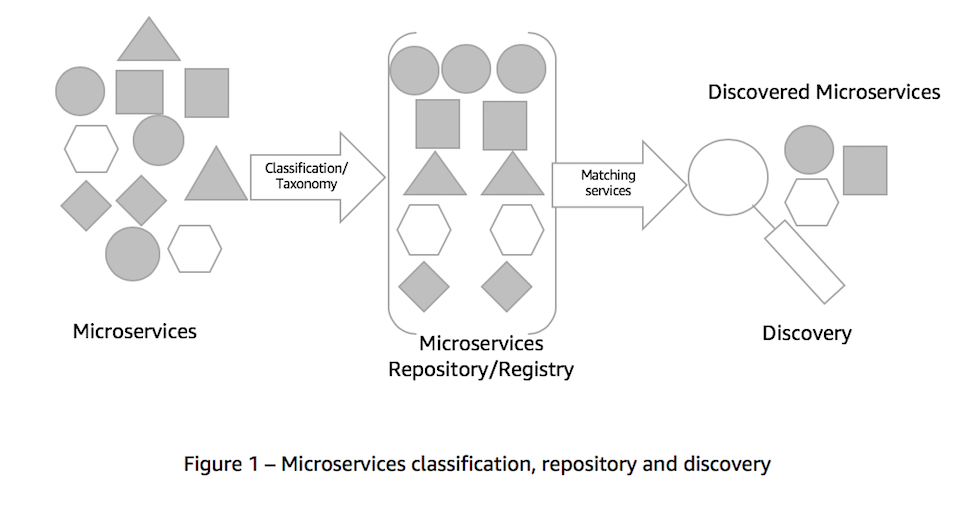
\includegraphics{microservices_classification.png}
\caption{Microservices classification.}
\end{figure}

\begin{figure}[!ht]
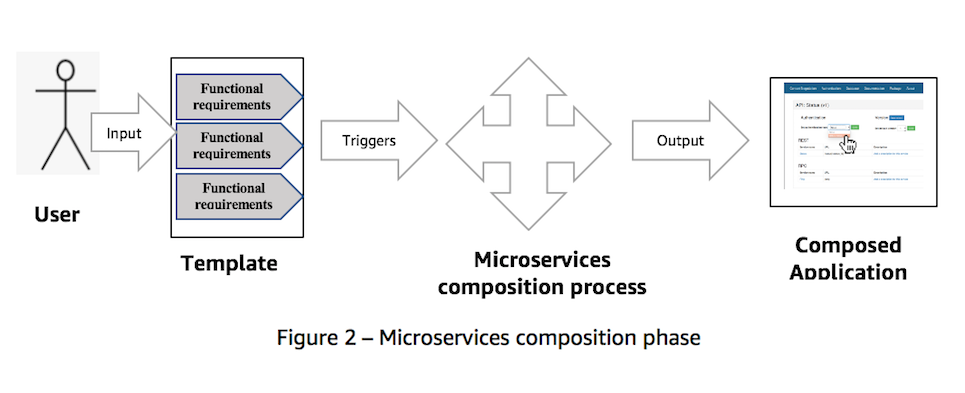
\includegraphics{microservices_composition.png}
\caption{Microservices composition.}
\end{figure}

\section{Project work packages}

The project will be broken down into the following work packages:

\begin{enumerate} 

\item \textbf{Classification}

The classification process will help with identification and grouping of microservices based on common properties. This will requires identifying the right semantics and producing a taxonomy to enable the classification process. 

\item \textbf{Repository and Registry}

In order to enable the discovery of microservices there would need to be stored into some type of repository with their attributes saved into some sort of registry, which the discovery engine can query to retrieve those microservices that meet the query criteria. 

\item \textbf{Discovery module}

The discovery module as its name implies will serve the purpose of discovering microservices prior to their composition into the desired application taking place. The discovered microservices will be persisted into a buffer or temporary storage before being processed 

\item \textbf{User input module}

In order for user to obtain a specific functionality powered by a specific service or set services, he or she will be required to provide a number of specifications in plain in English as input. This process may be guided that is a user is restricted to specific type of inputs (e.g. an input form with specified attributes that need to be filled or menu selections), or completely open meaning user have the freedom to type any text they want to express their requirements and the model will interpret their inputs to produce the needed functionality in the form of coordinated microservices. The decision to use a guided or open approach for user inputs will depend on the complexity and the feasibility of one over the other within the scope of this project which means that one approach may constitute an opportunity for further research.

\item \textbf{Execution module}

This module is the component that is responsible for the execution of composition of the discovered microservices and ultimately produce the composed application, which is expected to fulfill the user’s requirements.

\end{enumerate}

\section{Project Plan}

\begin{figure}[h!]
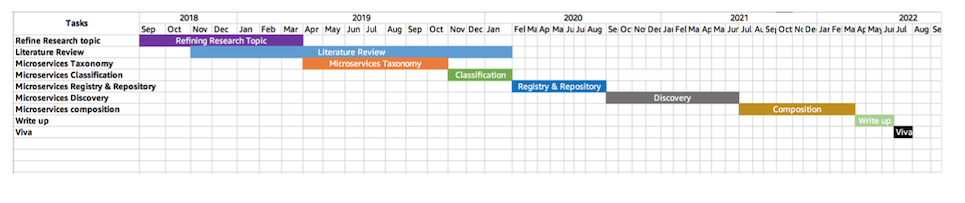
\includegraphics{project_plan.png}
\caption{Research project plan}
\end{figure}

\section{Progress report}
Table 1 below shows a report of the progress made on the research, while table 2 shows a list of trainings \& seminars that I have attended so far, and lastly table 3 contains all the meetings I have had with my supervisors.

\begin{table}[h!]
\begin{tabular}{|l|l|l|}
%\cline{1-3}
\hline
\textbf{\makecell[l]{Activity}} & \textbf{\makecell[l]{Status}} & \textbf{\makecell[l]{Comment}} \\ 
\hline
\makecell[l]{Literature review – Part 1} & \makecell[l]{Completed (See appendix)} & \makecell[l]{}\\ 
\hline
\makecell[l]{Taxonomy  \& classification \\of microservices paper} & \makecell[l]{In progress (See appendix)} & \makecell[l]{Currently refining\\ the methodology}\\ 
\hline
\makecell[l]{Microservices repository and registry} & \makecell[l]{Not started} & \makecell[l]{}\\ 
\hline
\makecell[l]{Microservices discovery} & \makecell[l]{Not started} & \makecell[l]{}\\ 
\hline
\makecell[l]{User input module} & \makecell[l]{Not started} & \makecell[l]{}\\ 
\hline
\makecell[l]{Microservices composition} & \makecell[l]{Not started} & \makecell[l]{}\\ 
\hline
\end{tabular}
\caption{Research progress report}
 \label{tab:Table 1}
\end{table}

\begin{table}[h!]
%\tiny
\begin{tabular}{|l|l|}
%\begin{tabular}{|l|l|}
\hline
\textbf{Training} & \textbf{Date}\\ 
\hline
 \makecell[l]{Research Integrity (Training)} & \makecell[l]{Completed on 5th Aug. 2019}\\ 
\hline
 \makecell[l]{Neuroscience-inspired artificial intelligence: \\ a case study of the retina (Seminar)} & \makecell[l]{Attended on 5th Oct. 2018}\\ 
\hline
 \makecell[l]{Failing with Style: Why and How we Should Encourage Humans to \\Fail with Highly Capable Systems (Seminar)} &\makecell[l]{ Attended on 12th Oct. 2018}\\ 
\hline
 \makecell[l]{Digital processes: correctness, compliance \\ and adoption considerations (Seminar)} &\makecell[l]{ Attended on 19th Oct. 2018}\\ 
\hline
 \makecell[l]{Generating C from Scala} & \makecell[l]{Attended on 26th Oct. 2018}\\ 
\hline
 \makecell[l]{Logical characterization of hybrid conformance (Seminar)} & \makecell[l]{Attended on 15th Nov. 2018 }\\ 
\hline
 \makecell[l]{A New Linear Logic for Deadlock-Free \\Session Typed Processes (Seminar)} & \makecell[l]{Attended on 23rd Nov. 2018}\\ 
\hline
 \makecell[l]{Detection under UAV with Convolutional \\Neural Network (Seminar)} &\makecell[l]{ Attended on 18th Dec. 2018}\\ 
\hline
 \makecell[l]{Developing the Graph-based Methods \\for Optimizing Job Scheduling on Multicore Computers (Seminar)} &\makecell[l]{ Attended on 18th Jan. 2019}\\ 
\hline
 \makecell[l]{On Reversibility and Continuous Integration (Seminar)} & \makecell[l]{Attended on 25th Jan. 2019}\\ 
\hline
 \makecell[l]{AR Experience Capturing and Sharing (Seminar)} & \makecell[l]{Attended on 7th Feb. 2019}\\ 
\hline
 \makecell[l]{Synthesis to Rational Synthesis: \\a Game-Theoretic Approach (Seminar)} &\makecell[l]{ Attended on 29th Mar. 2019}\\ 
\hline
     \makecell[l]{Multi-objective search for effective testing \\of Cyber-Physical Systems (Seminar)} & \makecell[l]{Attended on 16th Sep. 2019}\\ 
    \hline
\end{tabular}
\caption{Trainings \& Seminars}
 \label{tab:Table 2}
\end{table}

\begin{table}[h!]
\tiny
\begin{tabular}{|l|l|l|}
\hline
\textbf{Date} & \textbf{Participants} & \textbf{Meeting details} \\ \hline
5th Oct. 2018 & \makecell[l]{Georges – Jose \& Mohammad} & \makecell[l]{Kick off meeting to discuss research idea. \\Supervisors felt that we needed to refine the research idea and scope the,project properly. \\Jose \& Mohammad encouraged me to attend the seminars }\\ \hline
16th Oct. 2018 & \makecell[l]{Georges – Jose \& Mohammad }& \makecell[l]{Discussed,the revised project outline. \\Mohammed \& Jose recommended breaking the,project \\down into work packages. Jose recommended that \\I setup a slack channel,and GitHub repo for better collaboration. \\Jose also introduced me to LateX,\\and encouraged me to learn and use it. }\\ \hline
16th Nov. 2018 & \makecell[l]{Georges – Jose \& Mohammad} & \makecell[l]{Reviewed draft proposal \\and supervisors provided guidance on how to refine the \\idea to make it relevant for PhD research} \\ \hline
3rd Dec. 2018 & \makecell[l]{Georges – Jose \& Mohammad} & \makecell[l]{Talked about the idea of putting together a survey\\ to get input from functional experts\\ in a target industry on how they utilize microservices \\and if and how the outcome of my research could help \\address challenges around building microservices based applications \\which could be automated by means of service composition} \\ \hline
20th Dec. 2018 & \makecell[l]{Georges – Mohammad} & \makecell[l]{Mohammad provided guidance on which information \\ to look for when discussing with subject matter experts \\and recommended doing some reading on how to conduct a survey.} \\ \hline
25th Jan. 2019 & \makecell[l]{Georges – Jose \& Mohammad} & \makecell[l]{Discussed,the possible options going forward given\\ the challenges I faced gathering,details information on specific industry\\ (pending a discussion I was going to,have with a colleague on \\Amazon Serverless Application Repository module).,\\One option being to focus on a specific industry where information on,\\microservices would be accessible. The other one being to \\define a research,problem only relevant in academia.} \\ \hline
15th Feb. 2019 & \makecell[l]{Georges – Jose \& Mohammad} & \makecell[l]{Looked at how service composition using Amazon SAR \\worked for a single microservices. Supervisors advised \\to manually compose two or more microservices\\ to get a better understanding of what is involved in the process\\ and potential challenges before looking at automating \\the process which should constitutes one work package of the research. \\Also advised to review existing literature on Service orchestration, \\Service choreography, Service composition, etc.} \\ \hline
25th March 2019 & \makecell[l]{Georges – Jose \& Mohammad} & \makecell[l]{Discussed existing service composition methods.\\ Jose found an interesting paper on Medley framework \\for service compositionwhich he recommended that I read.} \\ \hline
15th April 2019 & \makecell[l]{Georges – Jose \& Mohammad} & \makecell[l]{Jose \& Mohammed recommended looking into the\\ taxonomy of microservices suggesting it \\might even be an opportunity to publish}\\ \hline
2nd May 2019 & \makecell[l]{Georges – Jose \& Mohammad} & \makecell[l]{We discussed the structure of the taxonomy paper. \\Mohammad advised to look at how to identify a finer \\classification of webservices and microservices,\\Have you encountered any characteristics of webservices \\and microservices (and their composition)?,that may\\ be used to classify them further into some subclasses? }\\ \hline
7th May 2019 & \makecell[l]{Georges – Jose \& Mohammad} & \makecell[l]{Mohammad,and Jose provided feedback on my proposed structure \\for writing the taxonomy paper,and areas to focus on} \\ \hline
14th May 2019 & \makecell[l]{Georges – Jose \& Mohammad} & \makecell[l]{Supervisors recommended reading other taxonomy papers \\to get a better understanding on how taxonomies are written} \\ \hline
17th May 2019 & \makecell[l]{Georges – Jose \& Mohammad} & \makecell[l]{Mohammad recommended a number of journals \\for searching for good taxonomy papers. \\Some journals you could search in: EEE,Transactions on Software Engineering, \\ACM,Transactions on Software Engineering and Methods,\\ACM,Computing Surveys, and,Empirical,Software Engineering. \\Please, do search in these journals.} \\ \hline
6th June 2019 & \makecell[l]{Georges – Mohammed} & \makecell[l]{Reviewed new version of the taxonomy paper and \\provided feedback. Supervisors insisted \\on clearly outlining the research questions, \\use a rigorous methodology which should \\lead to,results credible results} \\ \hline
13th Aug. 2019 & \makecell[l]{Georges – Jose \& Mohammed} & \makecell[l]{Reviewed new version of the taxonomy document \\and provided feedback. Areas to improve: Methodology }\\ \hline
16th Aug. 2019 & \makecell[l]{Georges – Jose \& Mohammed} & \makecell[l]{Reviewed new version of the taxonomy document \\ and provided feedback. Areas to improve: Methodology} \\ \hline
24th Aug. 2019 & \makecell[l]{Georges – Jose \& Mohammed} & \makecell[l]{Reviewed new version of the taxonomy \\document and provided feedback} \\ \hline
2nd Sept. 2019 & \makecell[l]{Georges \& Jose} & \makecell[l]{Jose recommended that I should make my,explanations a bit more rigorous, \\thinking of how I can be more convincing,that my taxonomy is generalizable; \\2. Try to bring up a few points on the,applicability of the taxonomy \\and how someone who reads my work could use it,to identify microservices \\(maybe conjecture about how this could be automated,\\to help in automated composition - which would connect to the larger idea of my,work)} \\ \hline
5th Sept. 2019 & \makecell[l]{Georges \& Mohammad} & \makecell[l]{Mohammad recommended that I provided more clarity on the search strategy. \\More specifically, he stressed that I should remove the search for the related papers \\as it did not help answer the research questions.\\ He said he noted some improvements but insisted on improving the \\ methodology.} \\ \hline
16th Sept. 2019 & \makecell[l]{Georges \& Jose} & \makecell[l]{I shared with Jose my intent to try the option \\of using information retrieval/Latent Semantic Indexing (LSI)/code search \\which I read in some papers. Jose recommended doing a POC first \\to make sure that it works before using as methodology \\in the taxonomy paper.,We also discussed the Probation report and \\Jose requested that I prepared the report and sent it to him \\so we could aim for the report meeting to take place by end September.} \\ \hline
\end{tabular}
\caption{Supervisors' meetings}
 \label{tab:Table 3}
\end{table}
\end{document}

